\title{Programming Assignment 4}
\author{
	Aditya Gupta\\
	\underline{2015CSB1003}}
\date{\today}
\documentclass{article}
\usepackage{adjustbox}
\usepackage{amsmath}
\usepackage{float}
\usepackage{graphicx}
\begin{document}
\maketitle
\section{Planners for Block World}
\subsection{Introduction}
The goal of this lab was to implement a planning agent for solving Block World Problem wherein given $N$ blocks and actions to ``pick a block from table'', ``unstack a block from another block'', ``release a holding block'' and ``stack a holding block onto another block'' we were required to reach a goal state configuration from an initial state using three different planners, ``forward search planner'' with BFS and A*; ``goal stack planning''. The initial and final state is composed of propositions such as \verb|(on 1 2)| and \verb|(ontable 3)|. Each action is a transformation of these propositions which has some \verb|preconditions|, which when true allows us to perform that action and the \verb|effects| of that actions are unified with the current state and the negative literals removed. States are represented in PDDL.

\section{Forward Search using BFS}
\subsection{Introduction}
In this search the states are maintained in a queue (initially containing only the initial state) and then every time a element is taken from the queue and checked for satisfying the goals. If it does not satisfy the goals then all actions which are applicable on the current state are taken (after instantiation) and applied on the current state all resulting states pushed onto the queue, in this way we only see states which require equal number of actions from the starting state and we get the optimal solution (minimum number of steps).

\pagebreak
\subsection{Observations}
\begin{itemize}
\item \verb|1.txt| In this problem the planner finds the solution of length 10 in around 3 ms and the optimal solution.

\begin{figure}[H]
    \centering
    \begin{minipage}{0.45\textwidth}
        \centering
        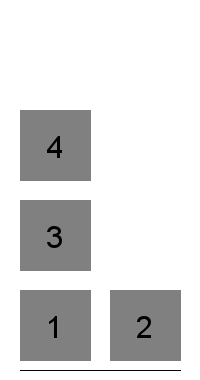
\includegraphics[scale=0.3]{1i}
        \caption{Initial State of 1.txt}
    \end{minipage}\hfill
    \begin{minipage}{0.45\textwidth}
        \centering
        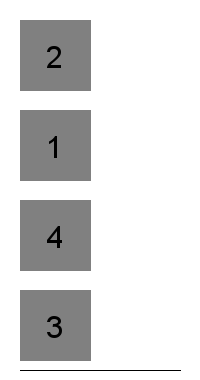
\includegraphics[scale=0.3]{1f}
        \caption{Final State of 1.txt}
    \end{minipage}
\end{figure}

\item \verb|4.txt| In this problem the planner finds the solution of length 14 in around 10ms and the optimal solution.

\begin{figure}[H]
    \centering
    \begin{minipage}{0.45\textwidth}
        \centering
        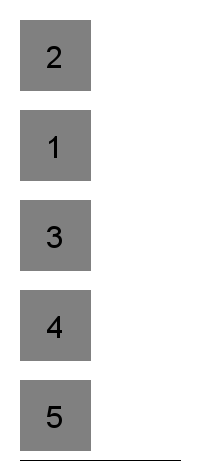
\includegraphics[scale=0.3]{4i}
        \caption{Initial State of 4.txt}
    \end{minipage}\hfill
    \begin{minipage}{0.45\textwidth}
        \centering
        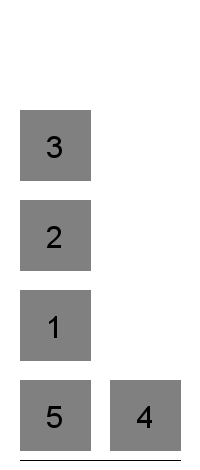
\includegraphics[scale=0.3]{4f}
        \caption{Final State  of 4.txt}
    \end{minipage}
\end{figure}
\end{itemize}

\section{Forward Search using A*}
\subsection{Introduction}
In this search the planner uses a priority queue instead of a normal queue where the the node with least $f$ value is taken where $f$ is given by:
$$f(n)=g(n)+h(n)$$
where $g$ is the level or depth of the current state, i.e. the total number of nodes takn until now and $h$ is the heuristic function. The heuristic function enables the search to be more directed towards the goal state and is faster and better than BFS. An optimal solution is returned only if the heuristic is admissible.
\subsection{Heuristic Function}
\subsubsection{H0: An Optimal One: Heights of Blocks}
In this heuristic the heights of the blocks in the current state is calculated. This is done via the following way:
\begin{itemize}
\item All the blocks on the table are given height 0, this can be done via finding propositions of type \verb|ontable b|.
\item For all possible blocks the block on it's top is found out and stored, this can be done via finding propositions of type \verb|on a b|
\item Finally the heights of all the blocks are given by starting with the ones on the ground via a BFS.
\end{itemize}
Now we relax the problem in this way: We can move any block from any height to its goal height by first holding it and then putting it, in most cases we either need to clear blocks from top of this or clear blocks on top of the goal block assuming it is in its correct position. So instead of taking these numerous steps we account for only 2 steps which will infact be the minimum. Also if we are holding a block currently we are halfway done so we only add 1 step. The heuristic value is thus the sum of 2 times blocks not currently at their goal height and 1 if we are holding a block.
\subsubsection{H1: An Unoptimal One: Relating to Number of Propositions}
\pagebreak
\subsection{Observations}
\begin{itemize}
\item \verb|2.txt| In this problem the $H0$ finds the solution of length 10 in again around 3ms and the optimal solution whereas the $H1$ finds the solution of length x in y ms which is not the optimal solution.(\textbf{Initial and final state same as} \verb|1.txt|)

\item \verb|6.txt| In this problem the $H0$ finds the solution of length 26 in around 4 min 4s and the optimal solution whereas the $H1$ finds the solution of length x in y ms which is not the optimal solution.

\begin{figure}[H]
    \centering
    \begin{minipage}{0.5\textwidth}
        \centering
        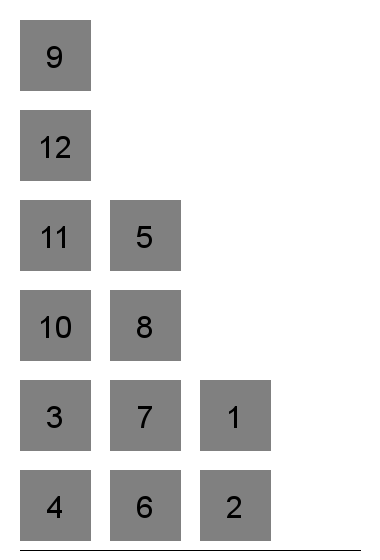
\includegraphics[scale=0.3]{6i}
        \caption{Initial State  of 6.txt}
    \end{minipage}\hfill
    \begin{minipage}{0.5\textwidth}
        \centering
        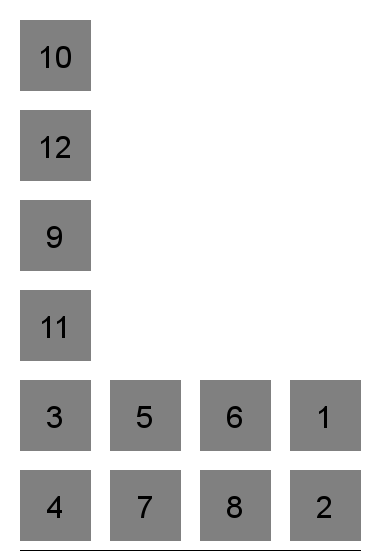
\includegraphics[scale=0.3]{6f}
        \caption{Final State  of 6.txt}
    \end{minipage}
\end{figure}
\end{itemize}

\section{Goal Stack Planning}
\subsection{Introduction}
In this search the planner tries to satisfy each goal one at a time assuming them as independently. It maintains a stack of propositions, goals and actions. First it puts all goals it wants to satisfy on the stack and then each proposition of it, then it tries to satisfy each proposition by choosing a relevant action disregarding whether the other propositions that it earlier tried to satisfy become false. After satisfying each of them one at a time it tries to see if each of them are true at the same time, if not it continues to try to satisfy each of its goal once again and so on. We see that it is wise to change the order of the goals to try different scenarios, probably skipping the first and putting it at the last. Also if it satisfies the conjunct goal it then performs the corresponding relevant action earlier chosen. 

A relevant action is one which results in the desired proposition being true and does not negate any goal. However we may get many relevant actions and the problem boils down to finding the most relevant action out of these.

\subsection{Selection of Relevant Action}
\subsubsection{S0: Most relevant action}
\subsubsection{S1: Maintaining count of used actions in particular situation and accounting relevancy}
This approach is based on making a {\bf general relevant action selection method for goal stack planning}. In this case we maintain count of every action returned by the ``relevant action'' selector function in a global structure corresponding to every state and proposition pair, i.e. for a given state and when trying to satisfy a given proposition which action was returned. Now our selection is based on returning the action which has least been used. This provides for all actions to be used equally. Also if there is a tie the action whose most preconditions are satisfied by the current state is taken. As a last resort every action has a chance of 1\% being selected  (may be replaced by another action if it satisfies any of these three conditions and is looked upon after this action) despite the number of times it has been used and the number of preconditions the current state satisfies. This ensures randomness and completeness. The results on large inputs is however too complex to be solved using this method. Also if by any chance the current state becomes the goal state and there are unnecessary goals and actions on the stack we short circuit the method to end there.
\subsubsection{S2: Manually Hardcoding the Relevant actions in form Goal-Action Conditions}
\pagebreak
\subsection{Observations}
\begin{itemize}
\item \verb|3.txt| In this problem $S0$ stucks into a loop as explained above, $S1$ finds the solution of length 10328 in around 568 ms and $S2$ finds the solution of length x in y ms.(\textbf{Initial and final state same as} \verb|4.txt|)

\item \verb|5.txt| In this problem ???(\textbf{Initial and final state same as} \verb|6.txt|)
\end{itemize}
\end{document}
